\documentclass[12pt,a4paper]{article}
\usepackage[utf8]{inputenc}
\usepackage[T1]{fontenc}
\usepackage{geometry}
\geometry{textwidth=6in}
\usepackage{amsmath}
\usepackage{amsfonts}
\usepackage{amssymb}
\usepackage{caption}
\usepackage{subcaption}
\usepackage{graphicx}
\usepackage{array}
\graphicspath{ {./images/} }
\usepackage{float}
% \usepackage{floatrow}
\usepackage{cancel}
\author{Paul Faugeras}
\date{Users' manual}
\title{Computer Vision Emergency Response Toolkit}
\renewcommand{\partname}

\begin{document}

\pagebreak

\begin{LARGE}
	\maketitle
\end{LARGE}

\pagebreak

\tableofcontents

\pagebreak

\part{Installation}

https://electronjs.org/docs/tutorial/support\#supported-platforms

\section{Windows}
\textbf{Requirements}\\
- Windows 7 or later,\\
- 400 Mb of free disk space.\\
~\\
The software has been tested (and ran smoothly) on 64-bit Windows 10 with 8Gb RAM, Intel Core i5 with potato GPU.\\
~\\
\textbf{Installation}\\
On the github page, use the links to download the \textbf{.exe} Windows installer. (please check your Windows distribution : you need the ia32 installer for x86 Windows, and x64 installer for amd64 Windows).\\
~\\
Double-click the installer, and follow the instructions.

\section{MacOS}
\textbf{Requirements}\\
- macOS 10.10 (Yosemite) or later,\\
- TBD of free disk space.\\
~\\
\textbf{Installation}\\
On the github page, use the links to download the \textbf{.dmg} MacOS installer.\\
~\\
Double-click the installer, and follow the instructions.


\section{Linux}
\textbf{Requirements}\\
- Ubuntu 12.04 or above, Fedora 21, Debian 8,\\
- 400 Mb of free disk space.\\
~\\
The software has been tested (and ran smoothly) on 64-bit Ubuntu 18.04 with 8Gb RAM, Intel Core i5 with potato GPU.\\
~\\
\textbf{Installation}\\
On the github page, use the links to download the Linux files.\\
~\\
You're on Linux (I like you), you know what to do...\\
~\\
\textit{Please note that both installers and standalone apps are available for Linux.}

\pagebreak

\part{User Interface}
\setcounter{section}{0}

\begin{figure}[H]
	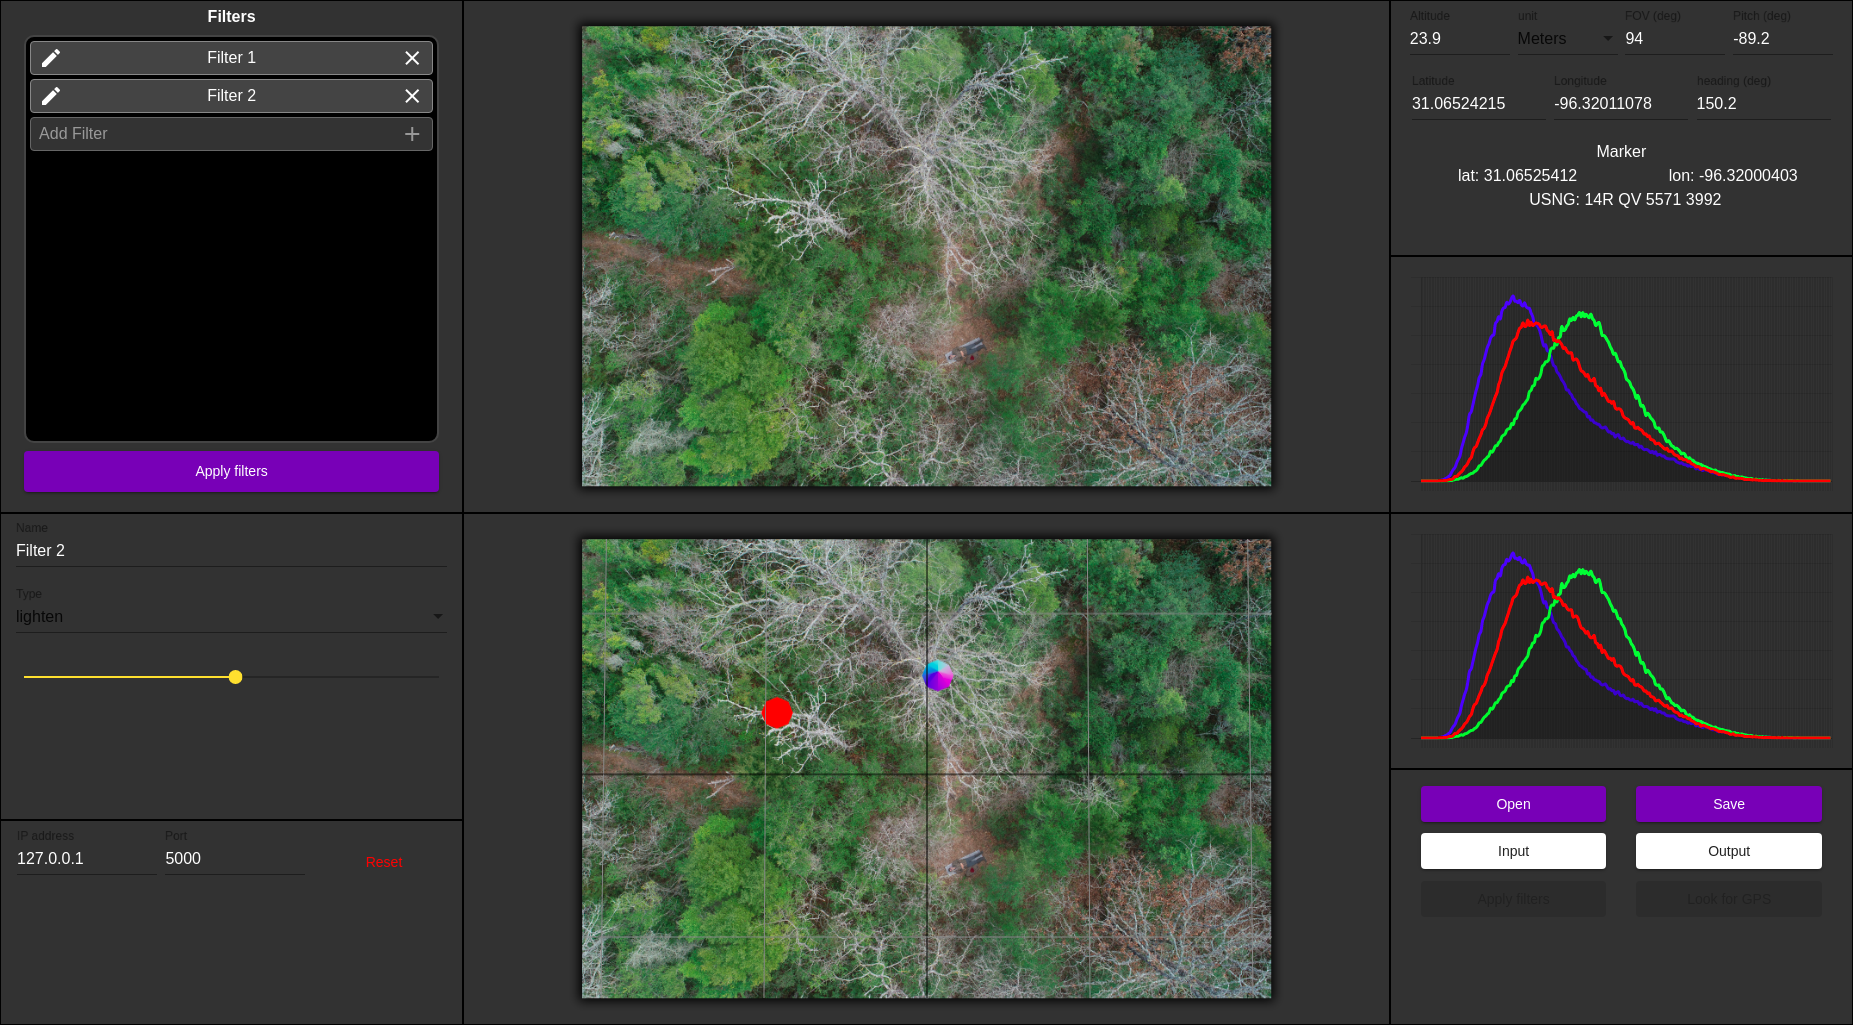
\includegraphics[scale=0.25]{user_interface}
	\centering
\end{figure}

\begin{itemize}
	\item \textbf{Top-left :} Current filters list,
	\item \textbf{Middle-left :} Selected filter edit,
	\item \textbf{Lower-left :} Back-end server settings (for developers only)
	\item \textbf{Top-center :} Currently opened image,
	\item \textbf{Lower-center :} Edited image (+ GIS grid and markers),
	\item \textbf{Top-right :} GIS settings and marker position,
	\item \textbf{Middle-right :} Top and bottom image histograms,
	\item \textbf{Lower-right :} Action buttons.
\end{itemize}

\part{Basic actions}
\setcounter{section}{0}

Basic actions are the first actions that you will use when running the software. For that, you will have to use the different buttons on the Action tab (lower right).

\begin{figure}[H]
	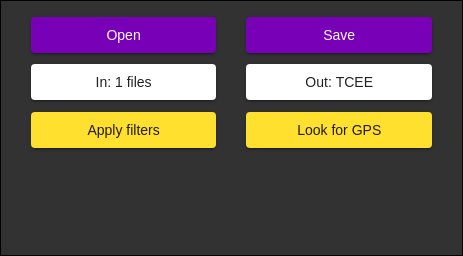
\includegraphics[scale=0.6]{action_tab}
	\centering
\end{figure}

\section{Opening and saving images}

To open an image, click on the button 'Open', and navigate to the desired file. Supported file types include JPEG, PNG, BMP, TIFF and GIF.\\
~\\
Once the image is opened, both the top and bottom image on the center panel should appear, with a grid overlay on the bottom image. The histograms should also appear.\\
~\\
After opening an image, the 'save' button should be clickable. After clicking on it, you will be prompted to choose a destination folder and file name to save the image. Please keep in mind for later that this action will save \textbf{the bottom picture}. You will see below that this will be the filtered image.

\section{Setting GIS data}

After opening an image, if the software finds DJI's metadata (exif-XMP) in the file, the GIS tab (top-right tab) will have updated all the informations that it found. Those include : the position the picture was taken at (latitude, longitude, altitude) as well as the camera orientation (gimbal pitch and heading). You can switch between meters and feet for the altitude.\\
~\\
Please kindly note that \textbf{you will have to manually set the diagonal Field Of View of the camera} (FOV), since DJI doesn't store that piece of information in the metadata.\\
~\\
If the software doesn't find any metadata in the image, default data will be used, but you can tune them manually.\\
~\\
Please kindly note that DJI's metadata are not extremely precise : you might have to tweak the settings manually until the grid overlay on the bottom image fits the displayed image.

\section{GIS Marker}

Once you are happy with the grid overlay fit on the bottom image, you can hover your mouse over the bottom image. You will notice a colored cone moving around on the grid plane : that is your current mouse position relative to the ground.

\begin{figure}[H]
	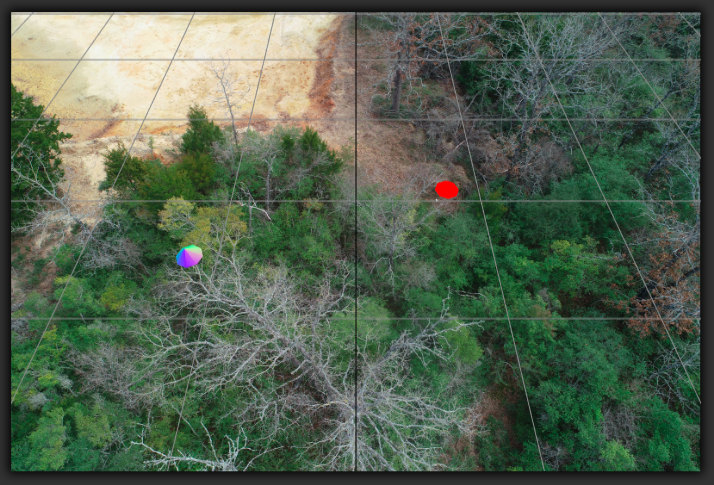
\includegraphics[scale=0.4]{grid}
	\centering
\end{figure}

After clicking on a spot on the image, you will see appear a red cone : that is your current marker position. On the GIS tab, you will see new fields appear : that will be your current marker's position : latitude, longitude and corresponding USNG coordinates.

\begin{figure}[H]
	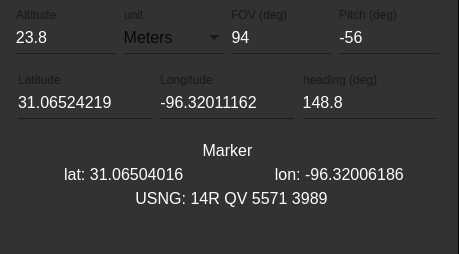
\includegraphics[scale=0.6]{gis}
	\centering
\end{figure}

You can update the current marker's position by clicking on an other spot on the image. The GIS tab will update accordingly. Please note that this marker will be the position selected when applying bulk GIS fetch (see below).

\pagebreak

\part{Filters}
\setcounter{section}{0}

The main function of this software is to apply filters to the open images. You can apply multiple filters in series to a single image, or to a whole bulk of images. More on that later.

\begin{figure}[H]
	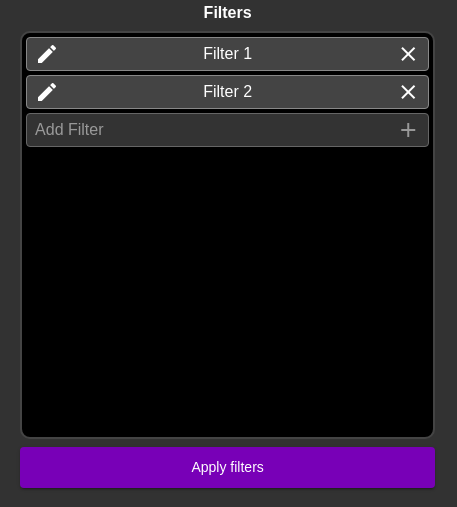
\includegraphics[scale=0.47]{filters_list}
	\centering
\end{figure}

\section{Adding, ordering and removing filters}

 Your curreent filters list is located in the top-left tab.\\
 ~\\
 The list is initialized empty. You can add a filter by clicking on the '+' button of the 'Add filter' item. This will add a default filter.\\
 ~\\
 After you've added multiple filters, you can reorganize them by dragging and dropping the filter item up and down the list. When applying the filters list (see below), they will be applied from top to bottom. For example, in the list above, 'Filter 1' will be applied to the source image, then 'Filter 2' will be applied to the resulting image. The results from 'Filter 2' will then be displayed on the bottom image.\\
 ~\\
 You can then remove a fliter by clicking on the cross located on the right of the desired filter item.
 
\section{Editing filters}

You can select the filter you would like to edit by clicking on the left pen icon of the desired filter item in the filters list tab. That will open the edition options of the selected filters in the filter edit tab, just underneath the list.\\
~\\
All filters have two common fields : the name of the filter (user-defined, it will be the name displayed on the list, to help the user identify which filter is which), and the nature of the filter.\\
~\\
There are two types of filters : basic filters and advanced filters, which can be selected with the drop down menu, and which we will be discussing below.

\subsection{Basic filters}

Basic filters are filters that do standard image modifications, such as color corrections, enhancement, contrast, hue, saturation modifications etc.\\
~\\
Each of those filters has its own parameter(s), that you can set in the edit tab, using sliders, color palette and basic parameter selection.

\begin{figure}[H]
	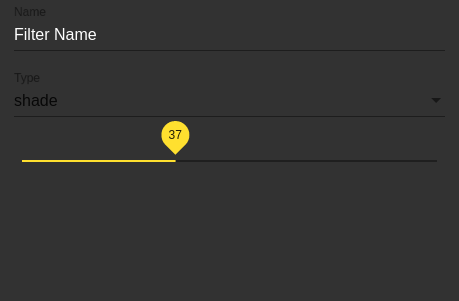
\includegraphics[scale=0.47]{simple_filter_edit}
	\centering
\end{figure}

\subsection{Advanced filters (server settings)}

Those filters are more advanced in the way that they apply computer vision algorithms to detect very specific features of an image.\\
~\\
Those algorithms are ran in the back-end through a Python instance. They use multiple settings, that you can edit by clicking on the 'Edit server settings' button (available in the filter edit tab when editing an advanced filter).\\

\begin{figure}[H]
	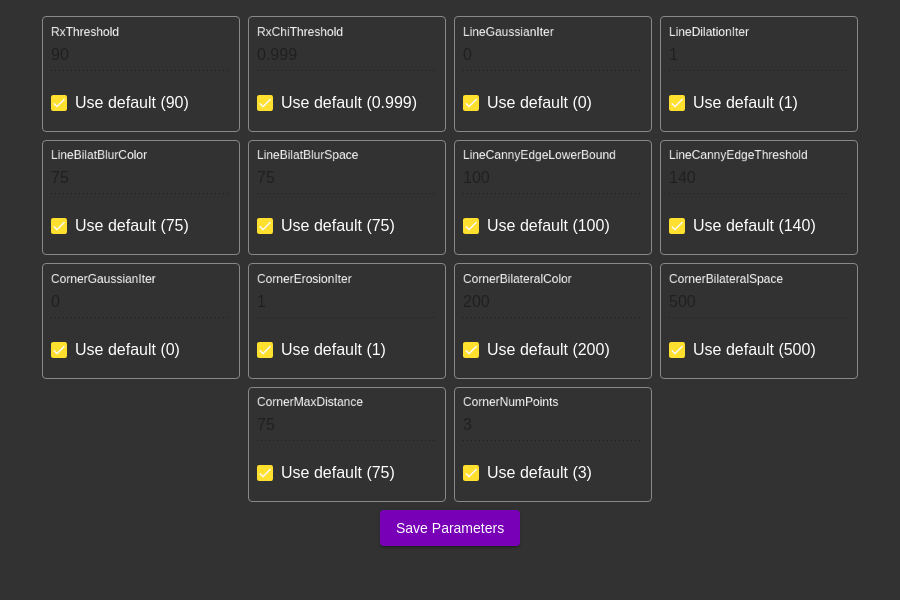
\includegraphics[scale=0.4]{advanced_settings}
	\centering
\end{figure}

From this window, you can select whether you would like to use the default value for each setting, or specify your own (which you can manually set).\\
~\\
Don't forget to save the parameters( by clicking on the button) before exiting!\\
~\\
Please also note that if you have multiple advanced filters in your filters list, there will only be one instance of the server settings (they will all use the same settings). This is a feature we are working on).

\section{Applying filters}

Once you have created your filters list, ordered the filters item and updated all the settings, you are ready to apply them to your opened image!\\
~\\
To do so, you need to click on the 'Apply filters' button, in the filters list tab. You will need an opened image in order to apply the filters, otherwise the button will be greyed out.\\
~\\
Once all the filters have been ran on the image, the bottom image will be updated with the result. You will then be able to save it to your computer (using the 'Save' button of the action tab), or modify your filters, and re-apply them to the top image.\\
~\\
\textit{Please note that if you run a new filters list on the top image, the results from the previous run will not be saved. Make sure to save your result before running a new batch of filters.}\\
~\\
\textit{Please also note that depending on your filters list and the power of your computer, the image might take quite a bit of time to update.}

\pagebreak

\part{Bulk actions}
\setcounter{section}{0}

The CVERT software also allows you to execute some actions to multiplle files in a single run.

\section{Selecting source and target}

\subsection{Selecting source files}

In the action tab, you need to click on the 'Input' button. Then a prompt will ask you to select the image files to apply the actions on. Those files WILL NOT be modified, but copied, so you have no risk of losing the orign files.
You can select multiple image files (same file types support as when clicking on 'Open').\\
~\\
Once you have selected the desired files, you will see that the Input button display will have been updated with the number of files you have selected.

\subsection{Selecting output folder}

In the actio nab, you need to click on the 'Output' button. Then a prompt will ask you to select the destination folder, where the algorithm will save the image results, after executing the action.\\
~\\
We advise you to use an empty folder as destination, in order to avoid accidentally overwriting files.

\section{Actions}

By executing the followin actions, all the files selected as input will be copied, processed and saved in the destination folder.

\subsection{Bulk fiiltering}

In order for this button ('Apply filters') to be clickable, you need to have a valid filters list, valid input files and output folder.\\
~\\
When clicking on this button, the current filters list will be applied to all the input images, and the resulting images will all be saved in the output folder.

\subsection{Bulk GIS fetch}
In order for this button ('Look for GPS') to be clickable, you need to have a valid GIS marker position, valid input files and output folder.\\
~\\
The software will check all the input files for DJI metadata (position, camera orientation etc.) to check if the marker position overlays with any of the images. If so, it will add a marker to the image at the marker position, and write it to the destination folder.\\
~\\
Please note that the image will NOT be saved if no DJI metadata is found, or if the marker doesn't overlay with the image.\\
~\\
Please also note thatthe used FOV is the one set on the GIS tab (make sure you have updated it, and all images are taken from the same model of drone), and the GIS metadata for the input images cannot be manually modified. That may lead to a few imprecise results (a few meters max).

\pagebreak

\part{Notes and debug}
\setcounter{section}{0}

\paragraph{} You may notice a 'server' tab in the bottom left corner : that is the IP address and port to the advanced filters server. It is designed to be used only by developers. Please do not modify its settings. If you accidentally changed its settings, you can click on the 'reset' button right next to it to restore it to its default settings.\\

\paragraph{} In case you encounter a bug, you can open and close the developers tools, by pressing (at the same time) Ctrl+Shift+I. If yu read an error message, it might tell you how to solve the issue. If not, you can report the issue to us.

\end{document}
